\documentclass[12pt,a4paper]{article}
\usepackage{graphicx}
\usepackage{listings}
\usepackage{color}
\usepackage{hyperref}
\usepackage{geometry}
\usepackage{float}
\usepackage{caption}
\usepackage{subcaption}
\usepackage{tabularx}
\usepackage{booktabs}
\usepackage{svg}
\usepackage{hyperref}
\usepackage{url}

\geometry{margin=1in}

% Code listing style
\definecolor{codegreen}{rgb}{0,0.6,0}
\definecolor{codegray}{rgb}{0.5,0.5,0.5}
\definecolor{codepurple}{rgb}{0.58,0,0.82}
\definecolor{backcolour}{rgb}{0.95,0.95,0.92}

\lstdefinestyle{mystyle}{
    backgroundcolor=\color{backcolour},   
    commentstyle=\color{codegreen},
    keywordstyle=\color{magenta},
    numberstyle=\tiny\color{codegray},
    stringstyle=\color{codepurple},
    basicstyle=\ttfamily\footnotesize,
    breakatwhitespace=false,         
    breaklines=true,                 
    captionpos=b,                    
    keepspaces=true,                 
    numbers=left,                    
    numbersep=5pt,                  
    showspaces=false,                
    showstringspaces=false,
    showtabs=false,                  
    tabsize=2
}
\lstset{style=mystyle}

\title{CS256 Class Project Report: FPGA Tetris\\- Mustafa Albahrani}

\author{
    Mustafa Albahrani \\
    \texttt{mustafa.albahrani@kaust.edu.sa}
    \and
    Mohammad Alkhalifah\thanks{Contributed to the project implementation; however, this report is an individual submission} \\
    \texttt{mohammad.alkhalifah@kaust.edu.sa}
}

\date{\today}



\begin{document}

\maketitle
\newpage

\tableofcontents
\newpage

\section{Introduction}

\subsection{Project Background}
Tetris is a classic tile-matching puzzle game created by Alexey Pajitnov in 1985. The game involves manipulating falling geometric shapes known as \textit{tetrominoes}---each consisting of four square blocks---by rotating and positioning them to complete horizontal lines on a 10$\times$20 grid. When a line is completed, it is cleared from the board, and the game continues until pieces stack to the top of the playfield.

\subsection{Motivation for FPGA Implementation}
Implementing Tetris on an FPGA provides an excellent opportunity to explore digital design concepts that are difficult to encounter in software-only development:
\begin{itemize}
    \item \textbf{Real-Time Signal Generation}: The VGA display requires precise timing signals generated at 83.46 MHz, demanding cycle-accurate hardware design.
    \item \textbf{Concurrent Processing}: Unlike sequential software execution, hardware must simultaneously handle video output, user input, and game state updates across multiple clock domains.
    \item \textbf{Finite State Machine Design}: The game logic requires a complex FSM to manage piece spawning, movement, rotation with wall kicks, line clearing, and scoring.
    \item \textbf{Protocol Implementation}: Direct interfacing with VGA displays and PS/2 keyboards requires implementing timing-critical communication protocols in hardware.
\end{itemize}

\subsection{Project Objectives}
The goal of this project was to design and implement a fully functional Tetris game on an Artix-7 FPGA development board. The implementation uses SystemVerilog to describe the hardware logic for VGA video signal generation, PS/2 keyboard input processing, and game state management. The system interfaces with a VGA monitor for display output and a keyboard for player control.

\section{VGA Signaling Protocol}

\subsection{Understanding the VGA Standard}
VGA (Video Graphics Array) is an analog video transmission standard that controls display output through three color channels (Red, Green, Blue) and two synchronization signals:
\begin{enumerate}
    \item \textbf{Horizontal Sync (HSYNC)}: Signals the end of each horizontal line and triggers horizontal retrace.
    \item \textbf{Vertical Sync (VSYNC)}: Signals the end of each frame and triggers vertical retrace.
\end{enumerate}

The synchronization signals control the scanning mechanism. In traditional CRT displays, an electron beam was deflected across the phosphor screen, scanning from top-left across each row sequentially. Modern LCD displays emulate this timing for compatibility. The key insight is that video signal generation is inherently a time-critical operation---each pixel must be output at precisely the right moment.

\subsection{Timing Parameters}
For the target resolution of $1280 \times 800$ at 60 Hz, the system operates with a pixel clock of approximately 83.46 MHz~[1]. The complete scan includes both visible pixels and blanking intervals for retrace:

\begin{table}[H]
    \centering
    \begin{tabular}{|l|c|c|}
    \hline
    \textbf{Parameter} & \textbf{Horizontal} & \textbf{Vertical} \\ \hline
    Total Count & 1680 (0-1679) & 828 (0-827) \\ \hline
    Sync Pulse End & 135 & 2 \\ \hline
    Visible Start & 336 & 27 \\ \hline
    Visible End & 1615 & 826 \\ \hline
    \end{tabular}
    \caption{VGA Timing Parameters for 1280$\times$800 @ 60 Hz.}
    \label{tab:vga_timing}
\end{table}

\section{Sync Pulse and Timing Generation}

\subsection{Counter-Based Implementation}
The VGA timing logic is implemented in the \texttt{vga\_out} module using two counters: \texttt{hcount} for horizontal position and \texttt{vcount} for vertical position.

\begin{lstlisting}[language=Verilog, caption=VGA Counter Logic in vga\_out.sv]
// Parameters from README
localparam H_MAX = 1679;
localparam V_MAX = 827;

always_ff @(posedge clk) begin
    if (rst) begin
        hcount <= 0;
        vcount <= 0;
    end else begin
        if (hcount == H_MAX) begin
            hcount <= 0;
            if (vcount == V_MAX) begin
                vcount <= 0;
            end else begin
                vcount <= vcount + 1;
            end
        end else begin
            hcount <= hcount + 1;
        end
    end
end
\end{lstlisting}

The horizontal counter increments on every pixel clock cycle, resetting after reaching 1679. Each time \texttt{hcount} wraps around, the vertical counter increments, creating the raster scan pattern.

\subsection{Sync Signal Generation}
The synchronization pulses are generated by comparing counter values against threshold parameters:

\begin{lstlisting}[language=Verilog, caption=Sync Pulse Generation]
// HSYNC: Active Low (0 when hcount 0-135)
assign hsync = ~(hcount <= H_SYNC_END); // H_SYNC_END = 135

// VSYNC: Active High (1 when vcount 0-2)
assign vsync = (vcount <= V_SYNC_END);  // V_SYNC_END = 2
\end{lstlisting}

The synthesized schematic in Figure \ref{fig:vga_sch} shows the counter blocks and comparator logic that generates these timing signals.

\begin{figure}[H]
    \centering
    \includegraphics[width=1.0\textwidth]{Schematic/VGA_inst_pics/full_vga.png}
    \caption{Synthesized schematic of the VGA timing generator showing counters and sync comparators.}
    \label{fig:vga_sch}
\end{figure}

\section{Determining Pixel Coordinates}

\subsection{Active Area Detection}
Since the raw counters include blanking intervals where no visible pixels are output, we must identify when the beam is within the visible region:

\begin{lstlisting}[language=Verilog, caption=Active Area and Coordinate Calculation]
// Active Area Detection
assign active_area = (hcount >= H_VIS_START && hcount <= H_VIS_END) &&
                     (vcount >= V_VIS_START && vcount <= V_VIS_END);

// Current X and Y (relative to visible area)
always_comb begin
    if (active_area) begin
        curr_x = hcount - H_VIS_START;  // Offset by 336
        curr_y = vcount - V_VIS_START;  // Offset by 27
    end else begin
        curr_x = 0;
        curr_y = 0;
    end
end
\end{lstlisting}

The \texttt{curr\_x} and \texttt{curr\_y} outputs represent the current visible pixel position, ranging from (0,0) at the top-left to (1279,799) at the bottom-right. This coordinate system is used by the rendering pipeline to determine what color each pixel should be.

\section{Drawing Objects on Screen}

\subsection{Rendering Architecture}
Unlike software rendering that draws to a frame buffer, FPGA-based rendering must compute the color of each pixel in real-time as it is being output. The \texttt{draw\_tetris} module implements a pipelined rendering approach to meet the strict timing requirements of a single pixel clock cycle ($<$12ns).

\subsection{Multi-Stage Pipeline}
The rendering pipeline operates in multiple stages:

\begin{enumerate}
    \item \textbf{Stage 1: Region Detection} --- The current pixel coordinates are classified into screen regions: main game grid, next piece preview, hold area, score display, or border. This narrows down the decision space for subsequent stages.
    
    \item \textbf{Stage 2: Data Access} --- Based on the detected region, the system fetches the appropriate data from game state memory (board array, current piece position).
    
    \item \textbf{Stage 3: Grid Index Calculation} --- For pixels within the game grid, the grid cell coordinates are calculated from the pixel position.
    
    \item \textbf{Stage 4: Color Output} --- The final RGB color is determined based on the cell contents and sprite data.
\end{enumerate}

\begin{lstlisting}[language=Verilog, caption=Grid Drawing Logic in draw\_tetris.sv]
// Calculate Grid Indices
s1_grid_col <= (curr_x - GRID_X_START) / BLOCK_SIZE;
s1_grid_row <= (curr_y - GRID_Y_START) / BLOCK_SIZE;

// Check if block exists (+2 offset for hidden spawn rows)
if (display.data[s1_grid_row + 2][s1_grid_col].data != `TETROMINO_EMPTY) begin
    s2_cell_color_idx <= display.data[s1_grid_row + 2][s1_grid_col].data + 1;
end
\end{lstlisting}

\begin{figure}[H]
    \centering
    \begin{subfigure}[b]{1.0\textwidth}
        \centering
        \includegraphics[width=\textwidth]{Schematic/draw_inst_pics/region_detectoin.png}
        \caption{Region Detection Logic (Stage 1)}
    \end{subfigure}
    \\
    \begin{subfigure}[b]{1.0\textwidth}
        \centering
        \includegraphics[width=\textwidth]{Schematic/draw_inst_pics/sprit_output.png}
        \caption{Sprite Output Logic (Stage 4)}
    \end{subfigure}
    \caption{Rendering Pipeline Implementation: Region detection and sprite output stages.}
    \label{fig:draw_pipeline}
\end{figure}

\subsection{Sprite System}
The \texttt{block\_sprite} module stores a 16$\times$16 grayscale texture in ROM that gives blocks a beveled 3D appearance. During rendering, the brightness value from the sprite is multiplied by a per-piece color (Cyan for I-piece, Purple for T-piece, etc.) to produce the final RGB output. This allows a single sprite texture to be reused for all seven piece types, saving memory.

\section{Game Logic Design}

\subsection{Module Architecture}
The system is organized as a hierarchy of specialized modules:

\vspace{0.3cm}
\noindent
\begin{tabularx}{\textwidth}{@{} l X @{}}
\toprule
\textbf{Module} & \textbf{Description} \\
\midrule
\texttt{game\_top} & Top-level wrapper that generates all system clocks and handles clock domain crossing. \\[0.5em]

\texttt{vga\_out} & VGA timing generator producing sync pulses and pixel coordinates. \\[0.5em]

\texttt{game\_control} & Core FSM governing game flow, spawning, gravity, and line clearing. \\[0.5em]

\texttt{draw\_tetris} & Rendering engine that determines pixel colors based on game state. \\[0.5em]

\texttt{input\_manager} & Input processor implementing Delayed Auto Shift (DAS). \\[0.5em]

\texttt{check\_valid} & Collision detection for piece movement and rotation. \\[0.5em]

\texttt{ghost\_calc} & Calculates the ghost piece drop position. \\
\bottomrule
\end{tabularx}

\subsection{Clock Architecture}
The system uses five distinct clock domains to balance performance with protocol requirements:

\begin{itemize}
\item \textbf{100 MHz}: Main system clock from the FPGA board.
\item \textbf{83.46 MHz}: Pixel clock for VGA timing (generated via MMCM).
\item \textbf{50 MHz}: PS/2 clock for keyboard sampling with sufficient oversampling margin.
\item \textbf{25 MHz}: Game logic clock for the FSM to avoid timing violations.
\item \textbf{60 Hz}: Game tick for gravity and animations, matching the display refresh rate.
\end{itemize}

\begin{figure}[H]
    \centering
    \begin{subfigure}[b]{0.48\textwidth}
        \centering
        \includegraphics[width=\textwidth]{Schematic/game_top_pics/clk_section.png}
        \caption{Clock Generation Circuit}
    \end{subfigure}
    \hfill
    \begin{subfigure}[b]{0.48\textwidth}
        \centering
        \includegraphics[width=\textwidth]{Schematic/game_top_pics/cdc_section.png}
        \caption{CDC Synchronizers}
    \end{subfigure}
    \caption{Clock Architecture and Domain Crossing Logic.}
    \label{fig:clock_arch}
\end{figure}

\subsection{Finite State Machine}
The game behavior is governed by a central FSM in \texttt{game\_control.sv} . Figure \ref{fig:fsm} shows the state transition diagram.

\begin{figure}[H]
    \centering
    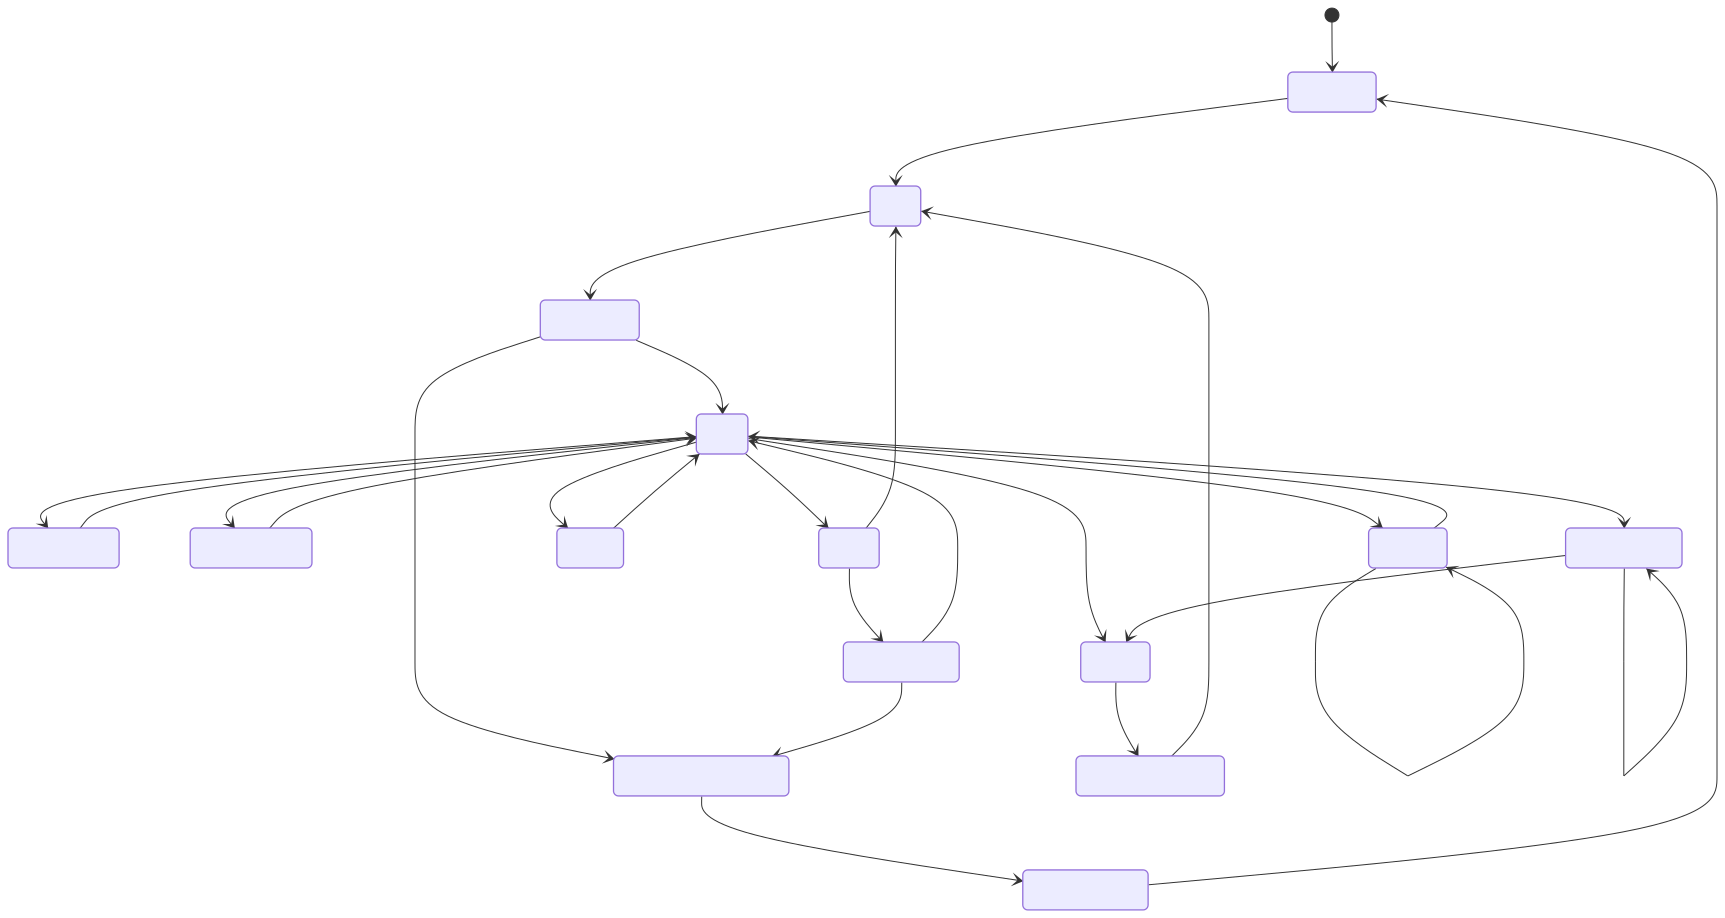
\includegraphics[width=1\textwidth]{fsm_diagram.png}
    \caption{Game Control FSM Diagram showing major state transitions.}
    \label{fig:fsm}
\end{figure}

\begin{table}[H]
    \centering
    \begin{tabular}{|l|l|}
    \hline
    \textbf{State} & \textbf{Description} \\ \hline
    \texttt{GEN} & Spawns a new tetromino from the 7-bag randomizer. \\ \hline
    \texttt{IDLE} & Waits for user input or gravity timer. \\ \hline
    \texttt{MOVE\_*} & Updates piece position and checks for collisions. \\ \hline
    \texttt{ROTATE} & Attempts rotation with SRS wall kicks. \\ \hline
    \texttt{DOWN} & Moves piece down; locks if blocked. \\ \hline
    \texttt{CLEAN} & Scans for and removes completed rows. \\ \hline
    \texttt{HOLD} & Swaps current piece with held piece. \\ \hline
    \texttt{GAME\_OVER} & Halts game until reset. \\ \hline
    \end{tabular}
    \caption{Description of Main FSM States.}
    \label{tab:fsm_states}
\end{table}

\subsection{7-Bag Randomizer}
To ensure fair gameplay, the \texttt{generate\_tetromino} module implements a 7-bag randomizer~[4]. Instead of pure random selection, the system shuffles all 7 piece types into a ``bag'' and draws from it sequentially. This guarantees that a player will never go more than 13 pieces without seeing any specific piece type.

\subsection{Super Rotation System (SRS)}
The project implements the Super Rotation System~[2] as defined in the Tetris Guideline~[3]. When a rotation would cause a collision, the system attempts up to 4 alternative ``kick'' offsets before rejecting the rotation. This allows players to rotate pieces even in tight spaces.

\subsection{T-Spin Detection}
Modern Tetris rewards advanced techniques like the T-Spin, where the T-piece rotates into a tight spot. The \texttt{spin\_detector} module checks if the piece is ``immobile'' (3 of 4 corners occupied) immediately after a rotation. If true and lines are cleared, bonus points are awarded. Figure \ref{fig:tspin_example} illustrates a typical T-Spin scenario.

\begin{figure}[H]
    \centering
    \includegraphics[width=0.6\textwidth]{tspin-example.jpg}
    \caption{Example of a T-Spin: The T-piece rotates into a slot where it is immobile.}
    \label{fig:tspin_example}
\end{figure}

\subsection{Ghost Piece}
The \texttt{ghost\_calc} module continuously calculates where the current piece would land if dropped instantly. This ``Ghost Piece'' is rendered semi-transparently to aid player accuracy. Figure \ref{fig:drop_rot} shows the hardware logic for the drop and rotate operations.

\begin{figure}[H]
    \centering
    \includegraphics[width=0.8\textwidth]{Schematic/game_inst/drop_rot.png}
    \caption{Logic for piece manipulation (Drop and Rotate).}
    \label{fig:drop_rot}
\end{figure}

\subsection{Input Processing}
The system supports both PS/2 keyboard and on-board pushbutton input. Figure \ref{fig:input_merge} shows how OR gates combine these sources.

\begin{figure}[H]
    \centering
    \includegraphics[width=0.8\textwidth]{Schematic/game_top_pics/input_mergingORs.png}
    \caption{Input merging logic combining keyboard and button inputs.}
    \label{fig:input_merge}
\end{figure}

The \texttt{input\_manager} module implements Delayed Auto Shift (DAS) for smooth movement controls. Dedicated counters track how long each direction key is held; after crossing a threshold, the system generates rapid movement pulses.

\begin{figure}[H]
    \centering
    \begin{subfigure}[b]{0.48\textwidth}
        \centering
        \includegraphics[width=\textwidth]{Schematic/input_mgr_pics/left0.png}
        \caption{Left DAS Counter}
    \end{subfigure}
    \hfill
    \begin{subfigure}[b]{0.48\textwidth}
        \centering
        \includegraphics[width=\textwidth]{Schematic/input_mgr_pics/right0.png}
        \caption{Right DAS Counter}
    \end{subfigure}
    \caption{Input Manager DAS Logic for Left/Right Movement.}
    \label{fig:input_das}
\end{figure}

\subsection{Resource Utilization}
The design was synthesized for the Artix-7 FPGA (xc7a100tcsg324-1). Table \ref{tab:utilization} summarizes the resource usage.

\begin{figure}[H]
    \centering
    \begin{subfigure}[b]{0.48\textwidth}
        \centering
        \includegraphics[width=\textwidth]{utilzation_bars.png}
        \caption{Utilization Bar Chart}
    \end{subfigure}
    \hfill
    \begin{subfigure}[b]{0.48\textwidth}
        \centering
        \includegraphics[width=\textwidth]{utilization_table.png}
        \caption{Utilization Table}
    \end{subfigure}
    \caption{FPGA Resource Utilization Summary.}
    \label{fig:utilization}
\end{figure}

\begin{table}[H]
    \centering
    \begin{tabular}{|l|r|r|r|}
    \hline
    \textbf{Resource} & \textbf{Utilization} & \textbf{Available} & \textbf{Utilization \%} \\ \hline
    LUT      & 25,787 & 63,400  & 40.67\% \\ \hline
    LUTRAM   & 2,004  & 19,000  & 10.55\% \\ \hline
    FF       & 3,941  & 126,800 & 3.11\%  \\ \hline
    BRAM     & 0.5    & 135     & 0.37\%  \\ \hline
    DSP      & 5      & 240     & 2.08\%  \\ \hline
    IO       & 41     & 210     & 19.52\% \\ \hline
    MMCM     & 1      & 6       & 16.67\% \\ \hline
    \end{tabular}
    \caption{FPGA Resource Utilization (Artix-7 xc7a100t).}
    \label{tab:utilization}
\end{table}

\section{Testing and Verification}

A comprehensive suite of testbenches was developed to verify individual modules before integration. All simulations were run in Vivado XSim.

\subsection{Testbench Summary}

\begin{table}[H]
    \centering
    \begin{tabular}{|l|l|c|}
    \hline
    \textbf{Testbench} & \textbf{Module Under Test} & \textbf{Result} \\ \hline
    \texttt{tb\_game\_control} & Core FSM (IDLE, MOVE, CLEAN) & 9/9 PASS \\ \hline
    \texttt{tb\_input\_manager} & DAS, one-shot logic & 17/17 PASS \\ \hline
    \texttt{tb\_rotate\_tetromino} & CW/CCW rotation matrix & 4/4 PASS \\ \hline
    \texttt{tb\_hold\_feature} & Hold swap, lockout & 9/9 PASS \\ \hline
    \texttt{tb\_generate\_tetromino} & 7-Bag randomizer & 13/13 PASS \\ \hline
    \texttt{tb\_vga\_out} & Sync pulse timing & Visual Pass \\ \hline
    \end{tabular}
    \caption{Summary of Testbenches and Results.}
    \label{tab:tb_summary}
\end{table}

\subsection{Game Control Simulation}
The core FSM was verified by simulating piece spawning, movement, rotation, hold functionality, and game over detection. Figure~\ref{fig:sim_waveform} shows a representative simulation waveform.

\begin{figure}[H]
    \centering
    \includegraphics[width=1.0\textwidth]{simulation_waveform.png}
    \caption{Simulation waveform from \texttt{tb\_game\_control} showing FSM state transitions and control signals.}
    \label{fig:sim_waveform}
\end{figure}

\subsection{Input Manager Testing}
The input manager testbench verified DAS timing and one-shot behavior for rotation commands:

\begin{verbatim}
Test 1: Rotate CW One-Shot
  PASS: Rotate CW Triggered on press
  PASS: Rotate CW Pulse Ended after one cycle
  PASS: Rotate CW did not re-trigger while holding

Test 4: Left DAS (Delayed Auto Shift)
  PASS: Left Initial Move on press
  PASS: No trigger during DAS delay (15 frames)
  PASS: Left DAS Auto-Repeat Triggered
\end{verbatim}

\subsection{Rotation Testing}
The rotation testbench verified clockwise and counter-clockwise matrix rotation:

\begin{verbatim}
Test 1: CW 0 -> 1
PASS: CW rotation 0 -> 1
Test 2: CW wrap 3 -> 0
PASS: CW rotation 3 -> 0
Test 3: CCW 0 -> 3
PASS: CCW rotation 0 -> 3
\end{verbatim}

\subsection{Hardware Validation}
On the physical Nexys A7-100T board, we verified:
\begin{itemize}
    \item \textbf{Visual Output}: The Tetris grid renders correctly with proper block colors.
    \item \textbf{Input Response}: DAS provides responsive, smooth controls similar to official Tetris games.
    \item \textbf{Gameplay}: Complete games were played including line clears, level progression, game over, and reset.
\end{itemize}

\section{References}

\begin{enumerate}

\item ``VESA Signal 1280 x 800 @ 60 Hz timing,'' tinyvga.com. [Online]. Available: \url{http://www.tinyvga.com/vga-timing/1280x800@60Hz}

\item ``Super Rotation System,'' TetrisWiki. [Online]. Available: \url{https://tetris.wiki/Super_Rotation_System}

\item ``Tetris Guideline,'' Hard Drop Tetris Wiki. [Online]. Available: \url{https://harddrop.com/wiki/Tetris_Guideline}

\item ``Random Generator,'' TetrisWiki. [Online]. Available: \url{https://tetris.wiki/Random_Generator}

\end{enumerate}

\section{Reflection}

This project provided valuable hands-on experience in digital design, bridging the gap between theoretical knowledge and practical hardware implementation for me. Working on a complete system from signal generation to game logic taught me how different components must integrate seamlessly.

\subsection{What I Enjoyed}
The most rewarding aspect was seeing the VGA output come to life on the monitor. Understanding how digital signals translate directly to visual information gave a tangible sense of accomplishment. Implementing the game logic was also satisfying, as it required carefully thinking through all possible states and edge cases and how to test them.

\subsection{Challenges Faced}
Clock domain crossing presented significant challenges. Ensuring that game state updates propagated correctly to the rendering pipeline without tearing or visual artifacts required careful synchronization. Debugging timing issues was particularly difficult since some problems only manifested on real hardware, not in simulation.

The Super Rotation System with wall kicks was more complex than initially anticipated. Implementing the lookup tables and testing all rotation scenarios across all piece types required systematic verification.

\subsection{What I Learned}
This project deepened my understanding of:
\begin{itemize}
    \item How VGA signaling works at the protocol level
    \item Designing pipelined architectures for real-time processing
    \item Managing multiple clock domains in a single design
    \item The importance of comprehensive testbenches for hardware verification
\end{itemize}

\subsection{Areas for Improvement}
If revisiting this project, I would invest more to integrate the FPGA board capibilities into the game (i.e. the different sensors etc.) to add on into the Tetris game. Also, I would love to play with the graphics more and make it a bit involved/complicated. We initially thought of making it two player game but we faced many issues with memory.

\subsection{Future Enhancements}
Potential improvements include:
\begin{itemize}
    \item Audio output using PWM for sound effects and music
    \item Animated score displays with visual effects for line clears
    \item Two-player competitive mode
    \item Customizable DAS settings and key mappings
\end{itemize}

\newpage
\appendix
\section{Appendix: Verilog Code}
This appendix contains the complete SystemVerilog source code for the AG Tetris project. Each file is prefaced with a brief description of its purpose.

% ==================== TOP LEVEL ====================
\subsection{Top Level Module}

\subsubsection*{game\_top.sv}
\textit{The main system integration module. It generates all required clock domains (83.46 MHz pixel, 50 MHz PS/2, 25 MHz game), instantiates all subsystems (VGA, input, game logic), and handles clock domain crossing between them.}
\lstinputlisting[language=Verilog]{game_top.sv}

% ==================== GLOBAL DEFINITIONS ====================
\subsection{Global Definitions}

\subsubsection*{GLOBAL.sv}
\textit{Shared header file containing game-wide constants such as grid dimensions (10$\times$20), tetromino type definitions, color indices, timing parameters, and custom data types used across all modules.}
\lstinputlisting[language=Verilog]{src/GLOBAL.sv}

% ==================== DISPLAY MODULES ====================
\subsection{Display Modules}

\subsubsection*{vga\_out.sv}
\textit{VGA timing generator. Produces horizontal/vertical sync pulses and active area signals for 1280$\times$800 resolution at 60 Hz. Outputs the current pixel coordinates (\texttt{curr\_x}, \texttt{curr\_y}) for the rendering pipeline.}
\lstinputlisting[language=Verilog]{src/display/vga_out.sv}

\subsubsection*{draw\_tetris.sv}
\textit{Main rendering engine. Implements a 4-stage pipeline to determine the color of each pixel by checking if it falls within the game grid, next piece preview, hold area, score display, or UI borders.}
\lstinputlisting[language=Verilog]{src/display/draw_tetris.sv}

\subsubsection*{block\_sprite.sv}
\textit{Sprite ROM for tetromino blocks. Stores a 16$\times$16 grayscale texture that is tinted with per-piece colors during rendering to give blocks a beveled 3D appearance.}
\lstinputlisting[language=Verilog]{src/display/block_sprite.sv}

\subsubsection*{draw\_number.sv}
\textit{Numeric digit renderer. Draws score and level numbers on screen by mapping digit values to a font ROM and outputting pixel data.}
\lstinputlisting[language=Verilog]{src/display/draw_number.sv}

\subsubsection*{draw\_string.sv}
\textit{Text string renderer. Draws static text labels ("SCORE", "LEVEL", "NEXT", "HOLD") on the game UI using a character ROM.}
\lstinputlisting[language=Verilog]{src/display/draw_string.sv}

\subsubsection*{seg7\_key\_display.sv}
\textit{7-segment display driver. Shows debug information (current key code, game state) on the FPGA board's 8-digit 7-segment display using time-multiplexed digit scanning.}
\lstinputlisting[language=Verilog]{src/display/seg7_key_display.sv}

% ==================== LOGIC MODULES ====================
\subsection{Game Logic Modules}

\subsubsection*{game\_control.sv}
\textit{Central game state machine. Implements the main FSM with 15 states governing piece spawning, movement, rotation (with SRS wall kicks), gravity, line clearing, hold functionality, and game over detection.}
\lstinputlisting[language=Verilog]{src/logic/game_control.sv}

\subsubsection*{generate\_tetromino.sv}
\textit{7-Bag randomizer. Generates tetromino pieces using the standard 7-bag algorithm, ensuring all 7 piece types appear exactly once before repeating.}
\lstinputlisting[language=Verilog]{src/logic/generate_tetromino.sv}

\subsubsection*{check\_valid.sv}
\textit{Collision detection. Checks if a proposed piece position is valid by testing for collisions with the field boundaries and locked blocks.}
\lstinputlisting[language=Verilog]{src/logic/check_valid.sv}

\subsubsection*{clean\_field.sv}
\textit{Line clearing logic. Detects complete rows, removes them, shifts all rows above downward, and returns the count of lines cleared for scoring.}
\lstinputlisting[language=Verilog]{src/logic/clean_field.sv}

\subsubsection*{create\_field.sv}
\textit{Field manipulation helper. Merges the current falling piece into the game field array when it locks in place.}
\lstinputlisting[language=Verilog]{src/logic/create_field.sv}

\subsubsection*{rotate\_tetromino.sv}
\textit{Rotation with wall kicks. Implements the Super Rotation System (SRS) by attempting standard rotation first, then trying up to 4 alternative kick offsets if collision occurs.}
\lstinputlisting[language=Verilog]{src/logic/rotate_tertomino.sv}

\subsubsection*{rotate\_clockwise.sv}
\textit{Basic rotation matrix. Performs a simple 90-degree clockwise rotation of a 4$\times$4 tetromino shape matrix.}
\lstinputlisting[language=Verilog]{src/logic/rotate_clockwise.sv}

\subsubsection*{ghost\_calc.sv}
\textit{Ghost piece calculator. Projects the current piece downward to find where it would land, enabling the semi-transparent "ghost" preview.}
\lstinputlisting[language=Verilog]{src/logic/ghost_calc.sv}

\subsubsection*{spin\_detector.sv}
\textit{T-Spin detection. Checks the 3-corner rule after T-piece rotations to determine if a T-Spin occurred for bonus scoring.}
\lstinputlisting[language=Verilog]{src/logic/spin_detector.sv}

\subsubsection*{bin\_to\_bcd.sv}
\textit{Binary to BCD converter. Converts binary score values to Binary-Coded Decimal for display on the 7-segment display.}
\lstinputlisting[language=Verilog]{src/logic/bin_to_bcd.sv}

% ==================== INPUT MODULES ====================
\subsection{Input Processing Modules}

\subsubsection*{ps2\_keyboard.sv}
\textit{PS/2 keyboard decoder. Processes raw scan codes from PS2Receiver, handles make/break prefixes (0xF0) and extended codes (0xE0), and outputs key events.}
\lstinputlisting[language=Verilog]{src/input/ps2_keyboard.sv}

\subsubsection*{PS2Receiver.sv}
\textit{Low-level PS/2 protocol handler. Samples the PS/2 clock and data lines to deserialize 11-bit frames (start, 8 data, parity, stop) into raw scan codes.}
\lstinputlisting[language=Verilog]{src/input/PS2Receiver.sv}

\subsubsection*{input\_manager.sv}
\textit{Input processing with DAS. Implements Delayed Auto Shift for smooth left/right movement and one-shot behavior for rotation, drop, and hold commands.}
\lstinputlisting[language=Verilog]{src/input/input_manager.sv}

\subsubsection*{debouncer.sv}
\textit{Button debouncer. Removes mechanical bounce from physical push-button inputs using a shift register and stability counter.}
\lstinputlisting[language=Verilog]{src/input/debouncer.sv}

% ==================== TESTBENCHES ====================
\subsection{Testbenches and Simulation Logs}

\subsubsection*{tb\_game\_control.sv}
\textit{Core FSM testbench. Verifies piece spawning, movement, rotation, hold functionality, hard drop, ghost position, and game over detection.}
\lstinputlisting[language=Verilog]{test/tb_game_control.sv}
\textbf{Simulation Log:}
\lstinputlisting[language={}]{test_logs/tb_game_control.log}

\subsubsection*{tb\_input\_manager.sv}
\textit{Input processing testbench. Tests Delayed Auto Shift (DAS) timing and one-shot behavior for rotation, drop, and hold commands.}
\lstinputlisting[language=Verilog]{test/tb_input_manager.sv}
\textbf{Simulation Log:}
\lstinputlisting[language={}]{test_logs/tb_input_manager.log}

\subsubsection*{tb\_rotate\_tetromino.sv}
\textit{Rotation testbench. Verifies clockwise and counter-clockwise rotation with SRS wall kick logic.}
\lstinputlisting[language=Verilog]{test/tb_rotate_tetromino.sv}
\textbf{Simulation Log:}
\lstinputlisting[language={}]{test_logs/tb_rotate_tertomino.log}

\subsubsection*{tb\_hold\_feature.sv}
\textit{Hold mechanic testbench. Tests piece swapping, hold lockout (preventing double-hold per piece), and edge cases.}
\lstinputlisting[language=Verilog]{test/tb_hold_feature.sv}
\textbf{Simulation Log:}
\lstinputlisting[language={}]{test_logs/tb_hold_feature.log}

\subsubsection*{tb\_generate\_tetromino.sv}
\textit{7-Bag randomizer testbench. Verifies that pieces are generated in valid range and follow the 7-bag algorithm.}
\lstinputlisting[language=Verilog]{test/tb_generate_tetromino.sv}
\textbf{Simulation Log:}
\lstinputlisting[language={}]{test_logs/tb_generate_teromino.log}

\subsubsection*{tb\_vga\_out.sv}
\textit{VGA timing testbench. Runs simulation over multiple frames to verify hsync, vsync, and active\_area signals.}
\lstinputlisting[language=Verilog]{test/tb_vga_out.sv}
\textbf{Simulation Log:}
\lstinputlisting[language={}]{test_logs/tb_vga.log}

\subsubsection*{tb\_ps2\_keyboard.sv}
\textit{PS/2 decoder testbench. Tests scan code processing including make/break detection and extended key codes.}
\lstinputlisting[language=Verilog]{test/tb_ps2_keyboard.sv}
\textbf{Simulation Log:}
\lstinputlisting[language={}]{test_logs/tb_ps2_keyboard.log}

\subsubsection*{tb\_PS2Receiver.sv}
\textit{Low-level PS/2 testbench. Verifies bit-level deserialization of PS/2 clock and data signals.}
\lstinputlisting[language=Verilog]{test/tb_PS2Receiver.sv}
\textbf{Simulation Log:}
\lstinputlisting[language={}]{test_logs/tb_PS2Receiver.log}

\end{document}
